% Options for packages loaded elsewhere
\PassOptionsToPackage{unicode}{hyperref}
\PassOptionsToPackage{hyphens}{url}
\PassOptionsToPackage{dvipsnames,svgnames,x11names}{xcolor}
%
\documentclass[
  letterpaper,
  DIV=11,
  numbers=noendperiod]{scrartcl}

\usepackage{amsmath,amssymb}
\usepackage{lmodern}
\usepackage{iftex}
\ifPDFTeX
  \usepackage[T1]{fontenc}
  \usepackage[utf8]{inputenc}
  \usepackage{textcomp} % provide euro and other symbols
\else % if luatex or xetex
  \usepackage{unicode-math}
  \defaultfontfeatures{Scale=MatchLowercase}
  \defaultfontfeatures[\rmfamily]{Ligatures=TeX,Scale=1}
\fi
% Use upquote if available, for straight quotes in verbatim environments
\IfFileExists{upquote.sty}{\usepackage{upquote}}{}
\IfFileExists{microtype.sty}{% use microtype if available
  \usepackage[]{microtype}
  \UseMicrotypeSet[protrusion]{basicmath} % disable protrusion for tt fonts
}{}
\makeatletter
\@ifundefined{KOMAClassName}{% if non-KOMA class
  \IfFileExists{parskip.sty}{%
    \usepackage{parskip}
  }{% else
    \setlength{\parindent}{0pt}
    \setlength{\parskip}{6pt plus 2pt minus 1pt}}
}{% if KOMA class
  \KOMAoptions{parskip=half}}
\makeatother
\usepackage{xcolor}
\setlength{\emergencystretch}{3em} % prevent overfull lines
\setcounter{secnumdepth}{2}
% Make \paragraph and \subparagraph free-standing
\ifx\paragraph\undefined\else
  \let\oldparagraph\paragraph
  \renewcommand{\paragraph}[1]{\oldparagraph{#1}\mbox{}}
\fi
\ifx\subparagraph\undefined\else
  \let\oldsubparagraph\subparagraph
  \renewcommand{\subparagraph}[1]{\oldsubparagraph{#1}\mbox{}}
\fi


\providecommand{\tightlist}{%
  \setlength{\itemsep}{0pt}\setlength{\parskip}{0pt}}\usepackage{longtable,booktabs,array}
\usepackage{calc} % for calculating minipage widths
% Correct order of tables after \paragraph or \subparagraph
\usepackage{etoolbox}
\makeatletter
\patchcmd\longtable{\par}{\if@noskipsec\mbox{}\fi\par}{}{}
\makeatother
% Allow footnotes in longtable head/foot
\IfFileExists{footnotehyper.sty}{\usepackage{footnotehyper}}{\usepackage{footnote}}
\makesavenoteenv{longtable}
\usepackage{graphicx}
\makeatletter
\def\maxwidth{\ifdim\Gin@nat@width>\linewidth\linewidth\else\Gin@nat@width\fi}
\def\maxheight{\ifdim\Gin@nat@height>\textheight\textheight\else\Gin@nat@height\fi}
\makeatother
% Scale images if necessary, so that they will not overflow the page
% margins by default, and it is still possible to overwrite the defaults
% using explicit options in \includegraphics[width, height, ...]{}
\setkeys{Gin}{width=\maxwidth,height=\maxheight,keepaspectratio}
% Set default figure placement to htbp
\makeatletter
\def\fps@figure{htbp}
\makeatother

\KOMAoption{captions}{tableheading}
\makeatletter
\makeatother
\makeatletter
\makeatother
\makeatletter
\@ifpackageloaded{caption}{}{\usepackage{caption}}
\AtBeginDocument{%
\ifdefined\contentsname
  \renewcommand*\contentsname{Table of contents}
\else
  \newcommand\contentsname{Table of contents}
\fi
\ifdefined\listfigurename
  \renewcommand*\listfigurename{List of Figures}
\else
  \newcommand\listfigurename{List of Figures}
\fi
\ifdefined\listtablename
  \renewcommand*\listtablename{List of Tables}
\else
  \newcommand\listtablename{List of Tables}
\fi
\ifdefined\figurename
  \renewcommand*\figurename{Figure}
\else
  \newcommand\figurename{Figure}
\fi
\ifdefined\tablename
  \renewcommand*\tablename{Table}
\else
  \newcommand\tablename{Table}
\fi
}
\@ifpackageloaded{float}{}{\usepackage{float}}
\floatstyle{ruled}
\@ifundefined{c@chapter}{\newfloat{codelisting}{h}{lop}}{\newfloat{codelisting}{h}{lop}[chapter]}
\floatname{codelisting}{Listing}
\newcommand*\listoflistings{\listof{codelisting}{List of Listings}}
\makeatother
\makeatletter
\@ifpackageloaded{caption}{}{\usepackage{caption}}
\@ifpackageloaded{subcaption}{}{\usepackage{subcaption}}
\makeatother
\makeatletter
\@ifpackageloaded{tcolorbox}{}{\usepackage[many]{tcolorbox}}
\makeatother
\makeatletter
\@ifundefined{shadecolor}{\definecolor{shadecolor}{rgb}{.97, .97, .97}}
\makeatother
\makeatletter
\makeatother
\ifLuaTeX
  \usepackage{selnolig}  % disable illegal ligatures
\fi
\IfFileExists{bookmark.sty}{\usepackage{bookmark}}{\usepackage{hyperref}}
\IfFileExists{xurl.sty}{\usepackage{xurl}}{} % add URL line breaks if available
\urlstyle{same} % disable monospaced font for URLs
\hypersetup{
  pdftitle={Ant Wars, Human Wars},
  pdfauthor={Graeme MacQueen; Tom Slee},
  colorlinks=true,
  linkcolor={blue},
  filecolor={Maroon},
  citecolor={Blue},
  urlcolor={Blue},
  pdfcreator={LaTeX via pandoc}}

\title{Ant Wars, Human Wars}
\author{Graeme MacQueen \and Tom Slee}
\date{1/1/23}

\begin{document}
\maketitle
\ifdefined\Shaded\renewenvironment{Shaded}{\begin{tcolorbox}[frame hidden, boxrule=0pt, breakable, interior hidden, borderline west={3pt}{0pt}{shadecolor}, enhanced, sharp corners]}{\end{tcolorbox}}\fi

\renewcommand*\contentsname{Contents}
{
\hypersetup{linkcolor=}
\setcounter{tocdepth}{3}
\tableofcontents
}
\hypertarget{ants-fight-wars}{%
\section{Ants fight wars}\label{ants-fight-wars}}

\hypertarget{ants-are-amazing}{%
\subsection{Ants are amazing}\label{ants-are-amazing}}

It's common knowledge that ant societies are remarkably complex, and
display many behaviours that are otherwise seen only in human societies.
They practice what looks like agriculture: some ants have gone beyond
hunting and foraging, and tend both crops (fungus) and animals (aphids,
caterpillars). Ants build settlements that are like cities, with waste
management systems, temperature control, road networks and defence
capabilities. And, of course, they fight what look like wars.

\hypertarget{weaver-ant-war-an-example}{%
\subsection{Weaver ant war: an
example}\label{weaver-ant-war-an-example}}

Let's get specific. Here is a two-minute video of David Attenborough
describing how weaver ants ``battle to protect their fortress'' in the
Australian tropical rain forest.

\url{https://youtu.be/SdpGAdB_zpc}

\hypertarget{weaver-ant-war-in-images}{%
\subsection{Weaver ant war: in images}\label{weaver-ant-war-in-images}}

And here, in case you don't want to watch the video, is David
Attenborough's narration together with some stills.

\begin{figure}

\begin{minipage}[t]{0.50\linewidth}

{\centering 

Narration: ``The rich territory of a successful colony draws \ldots{}
destructive enemies. Raiders from a neighbouring weaver ant colony
looking to expand their own empire\ldots{}''

}

\end{minipage}%
%
\begin{minipage}[t]{0.50\linewidth}

{\centering 

\raisebox{-\height}{

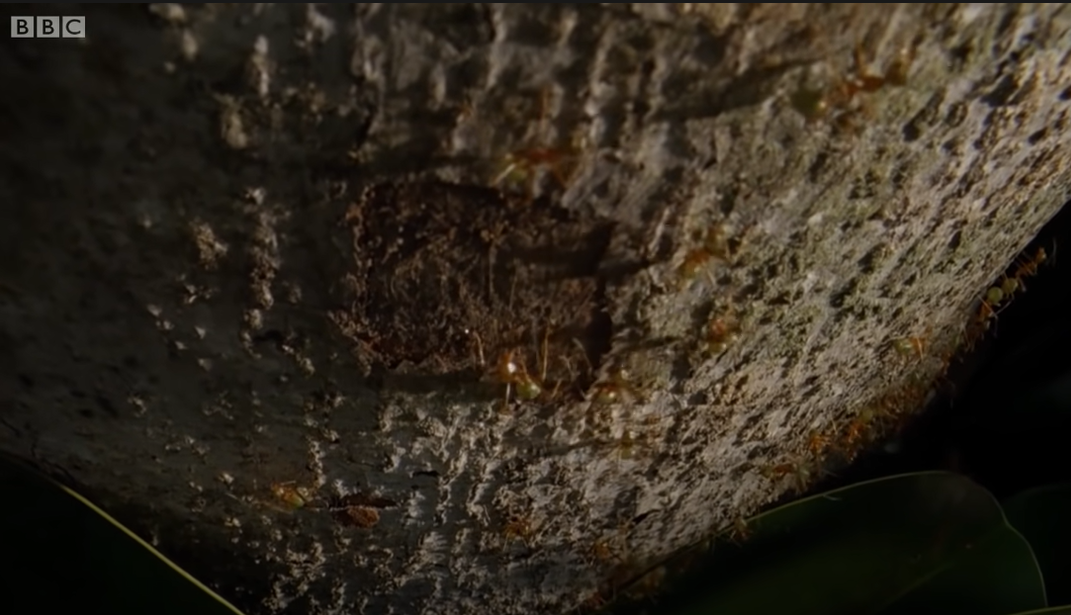
\includegraphics{weaver_ants_1.png}

}

\caption{\label{fig-weaver-ants-1}Raiders approach}

}

\end{minipage}%
\newline
\begin{minipage}[t]{0.50\linewidth}

{\centering 

Narration: ``Invaders are quickly spotted! The guard releases pheromones
to alert the rest of the colony.''

}

\end{minipage}%
%
\begin{minipage}[t]{0.50\linewidth}

{\centering 

\raisebox{-\height}{

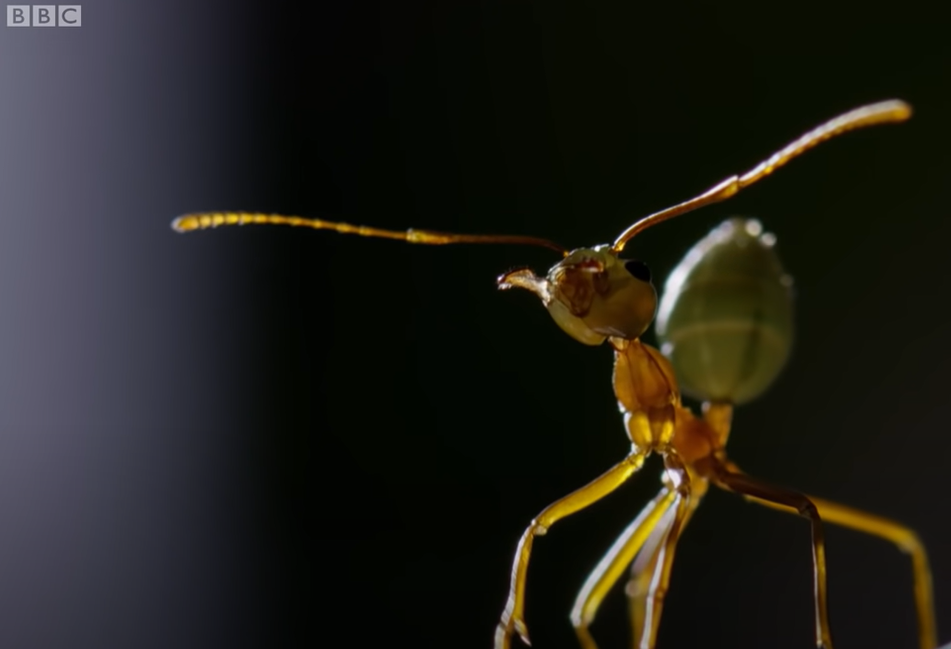
\includegraphics{weaver_ants_2.png}

}

\caption{\label{fig-weaver-ants-2}A guard sounds the alarm}

}

\end{minipage}%
\newline
\begin{minipage}[t]{0.50\linewidth}

{\centering 

Narration: ``They stream out of the nest to defend their home\ldots{}''

}

\end{minipage}%
%
\begin{minipage}[t]{0.50\linewidth}

{\centering 

\raisebox{-\height}{

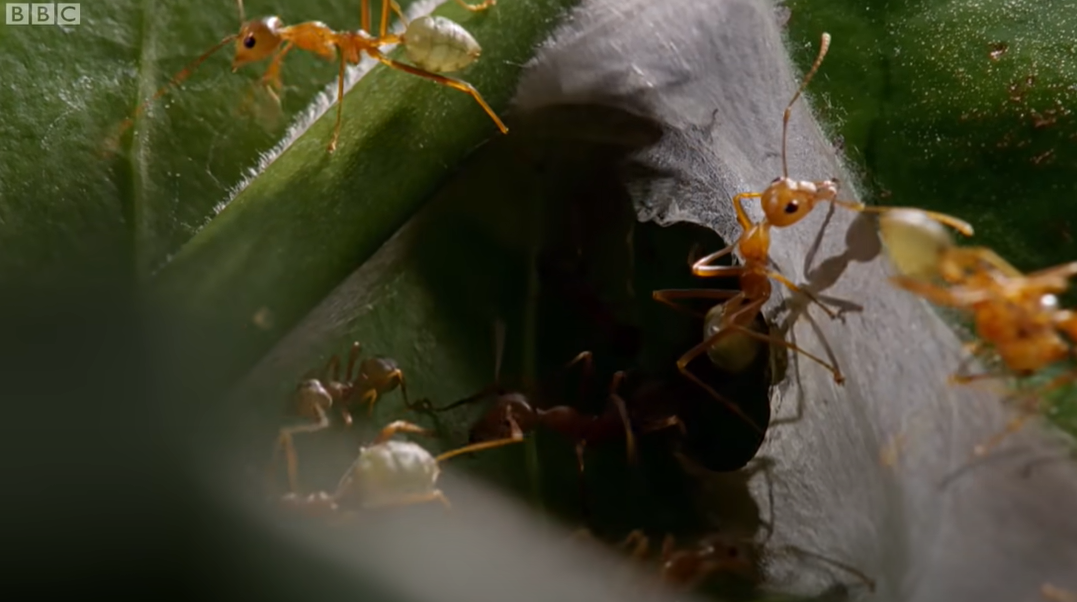
\includegraphics{weaver_ants_3.png}

}

\caption{\label{fig-weaver-ants-3}Ants rush to defend}

}

\end{minipage}%
\newline
\begin{minipage}[t]{0.50\linewidth}

{\centering 

Narration: ``If the home defences fail, the colony will be wiped out!''

}

\end{minipage}%
%
\begin{minipage}[t]{0.50\linewidth}

{\centering 

\raisebox{-\height}{

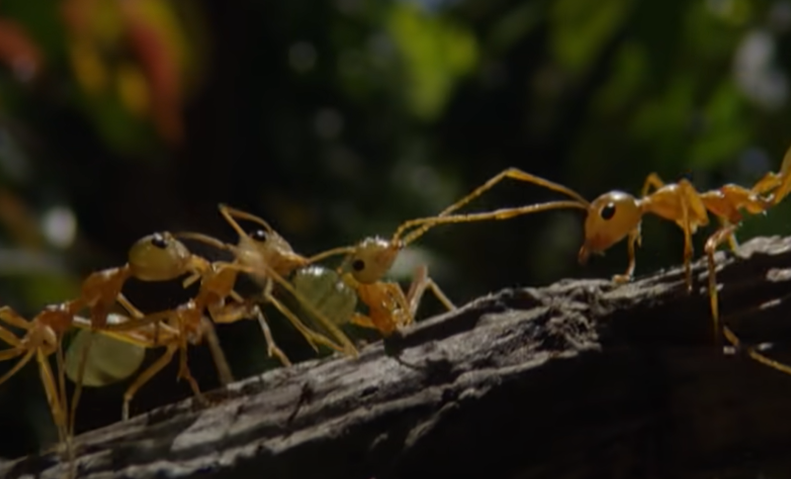
\includegraphics{weaver_ants_4.png}

}

\caption{\label{fig-weaver-ants-4}The colony is at stake}

}

\end{minipage}%
\newline
\begin{minipage}[t]{0.50\linewidth}

{\centering 

Narration: ``Some of the defenders deploy their most potent weapon. They
squirt formic acid. The stinging liquid halts the invaders in their
tracks.''

}

\end{minipage}%
%
\begin{minipage}[t]{0.50\linewidth}

{\centering 

\raisebox{-\height}{

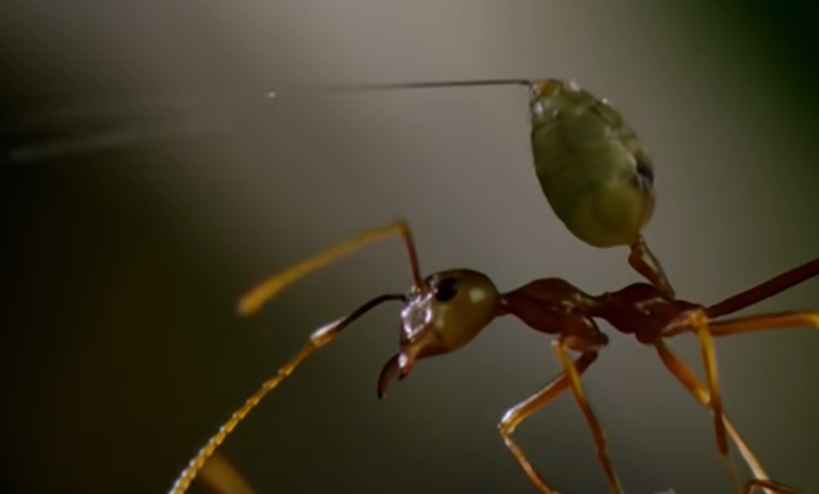
\includegraphics{weaver_ants_5.png}

}

\caption{\label{fig-weaver-ants-5}The defenders use weapons}

}

\end{minipage}%
\newline
\begin{minipage}[t]{0.50\linewidth}

{\centering 

Narration: ``And now the home guard can go on the offensive.''

}

\end{minipage}%
%
\begin{minipage}[t]{0.50\linewidth}

{\centering 

\raisebox{-\height}{

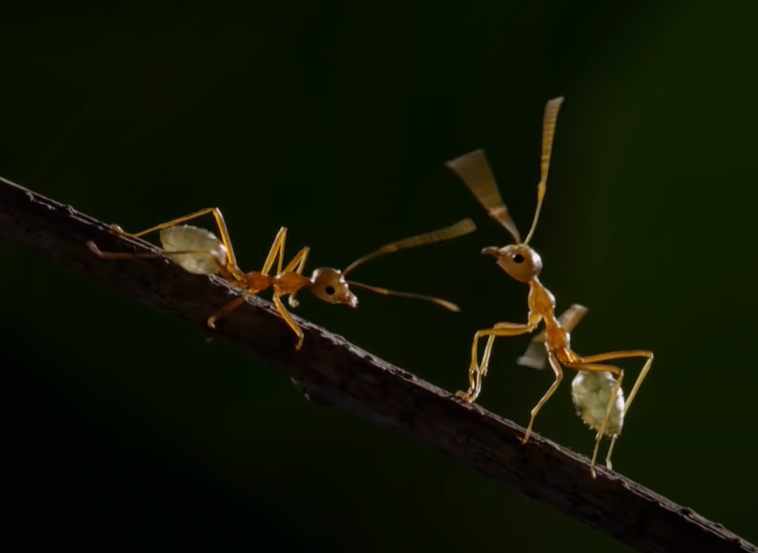
\includegraphics{weaver_ants_6.png}

}

\caption{\label{fig-weaver-ants-6}Defenders go on the attack}

}

\end{minipage}%
\newline
\begin{minipage}[t]{0.50\linewidth}

{\centering 

Narration: ``Home and territory are secure once again. A colony may lose
many workers in defence of its home, but their sacrifice helps safeguard
the next generation.''

}

\end{minipage}%
%
\begin{minipage}[t]{0.50\linewidth}

{\centering 

\raisebox{-\height}{

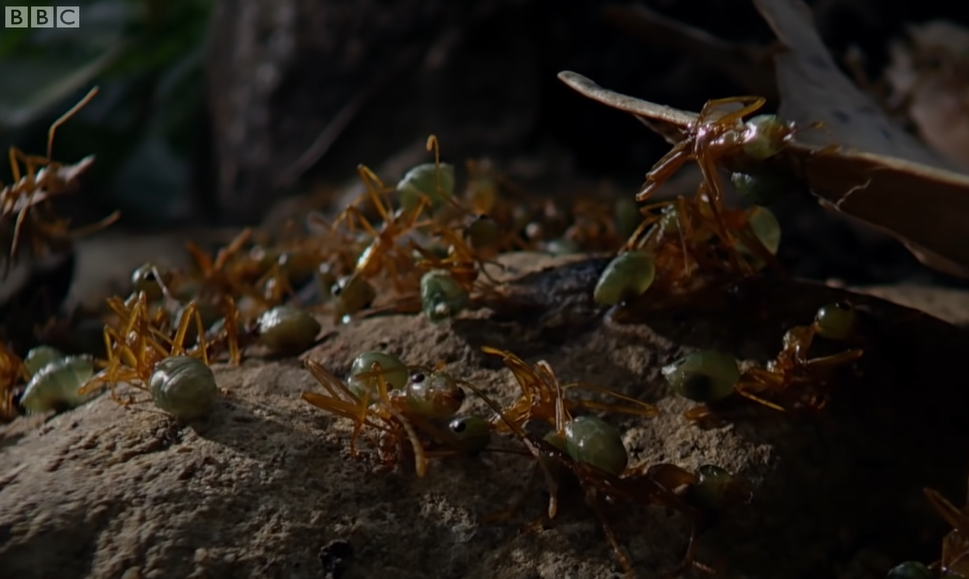
\includegraphics{weaver_ants_7.png}

}

\caption{\label{fig-weaver-ants-7}The defenders are victorious}

}

\end{minipage}%

\end{figure}

\hypertarget{definition-of-a-war}{%
\subsection{Definition of a war}\label{definition-of-a-war}}

This conflict not only looks like a war, it fits definitions of war
commonly used by social scientists. The Stanford Encyclopaedia of
Philosophy defines wars as ``large-scale armed conflicts between
organized groups''. International relations theorists use a very similar
definition: ``large-scale organized violence between political units''.
Let's take these one at a time.

\hypertarget{scale}{%
\subsubsection{Scale}\label{scale}}

Is the weaver ant conflict large scale? Yes. In some cases a colony may
be wiped out entirely, and that may involve the death of half a million
ants.

\hypertarget{organization}{%
\subsubsection{Organization}\label{organization}}

The war shows organization at several scales. Ants co-operate in teams
during combat. There are guards patrolling the borders of the colony:
they raise an alarm with a signal, and ants mobilize defences. Or they
attack as a group, as you can see. The society as a whole is organized,
with war fighting being one of the driving forces.

\hypertarget{armed}{%
\subsubsection{Armed}\label{armed}}

Humans extend our ability to kill by using weapons - tools or devices
separate from the body and extending its functions. Ant weapons are
organic, but make ant engagements deadly.

For the purposes of this article, we define a war as mass, organized,
mutual, and lethal conflict between communities.

\hypertarget{other-ant-wars}{%
\subsection{Other ant wars}\label{other-ant-wars}}

\begin{itemize}
\item
  Wood ants
\item
  Leafcutter ants
\item
  Argentine ants
\item
  Interspecies wars
\item
  Colony size and war
\end{itemize}

\hypertarget{so-what}{%
\subsection{So what?}\label{so-what}}

MacMillan (p xi): ``War raises fundamental questions about what it is to
be human and about the essence of human society''.

\hypertarget{when-we-think-about-war}{%
\section{When we think about war}\label{when-we-think-about-war}}

What do we talk about?

\hypertarget{political-science}{%
\subsection{Political science}\label{political-science}}

Weaver ants and territorial wars. Boundaries, neo-realist states,
investment decisions. Equilibria and shocks.

\hypertarget{in-group-out-group-theories}{%
\subsection{In-group / out-group
theories}\label{in-group-out-group-theories}}

Argentine ants

\hypertarget{the-militarized-state}{%
\subsection{The militarized state}\label{the-militarized-state}}

Social organization and investment

\hypertarget{diplomacy-and-intelligence-gathering}{%
\subsection{Diplomacy and intelligence
gathering}\label{diplomacy-and-intelligence-gathering}}

Tournaments, display,

\hypertarget{bright-lines-or-spectrum-of-conflict}{%
\section{Bright lines or spectrum of
conflict}\label{bright-lines-or-spectrum-of-conflict}}

\hypertarget{containing-war}{%
\subsection{Containing war}\label{containing-war}}

\begin{itemize}
\item
  At the individual level: behaviours, rituals, and separating war from
  peace. Even in war: ethics and the heroic warrior - bravery and
  courage.
\item
  At the societal level: institutions, discipline, War makes the state
  and the state makes war?
\item
  International: diplomacy, declarations, international law and
  conventions
\end{itemize}

\hypertarget{a-war-system}{%
\section{A war system}\label{a-war-system}}

\hypertarget{convergent-evolution}{%
\subsection{Convergent evolution}\label{convergent-evolution}}

\hypertarget{open-ended-questions-from-a-different-perspective}{%
\subsection{Open-ended questions from a different
perspective}\label{open-ended-questions-from-a-different-perspective}}



\end{document}
